\section{Detektorer -- Demodulatorer}
\textbf{HAREC a.\ref{HAREC.a.3.5}\label{myHAREC.a.3.5}}
\label{detektorer}
\index{detektor}
\index{demodulator}

\subsection{Allmänt}

Sändaren omvandlar informationen i lågfrekventa signaler till
högfrekvens som kan strålas ut från en antenn. I
mottagningsanläggningen återvandlas informationen, vilket kallas
demodulation eller demodulering.

I mottagare som är specialiserade för ett sändningsslag, används bara
en typ av demodulator medan mottagare för flera sändningsslag, AM,
SSB/CW, FM etc. har flera demodulatorer. Det finns många typer och
namn på demodulatorer, t.ex. detektor, diskriminator. Här beskrivs
några av dem.

\subsection{AM-detektorer}
\index{detektor!AM}
\index{AM!detektor}

\subsubsection{Dioddetektorn AM (A3E)}
\textbf{HAREC
  a.\ref{HAREC.a.3.5.1}\label{myHAREC.a.3.5.1},
  a.\ref{HAREC.a.3.5.2}\label{myHAREC.a.3.5.2}
}
\index{dioddetektor}
\index{AM!dioddetektor}
\index{A3E!dioddetektor}

\begin{figure}
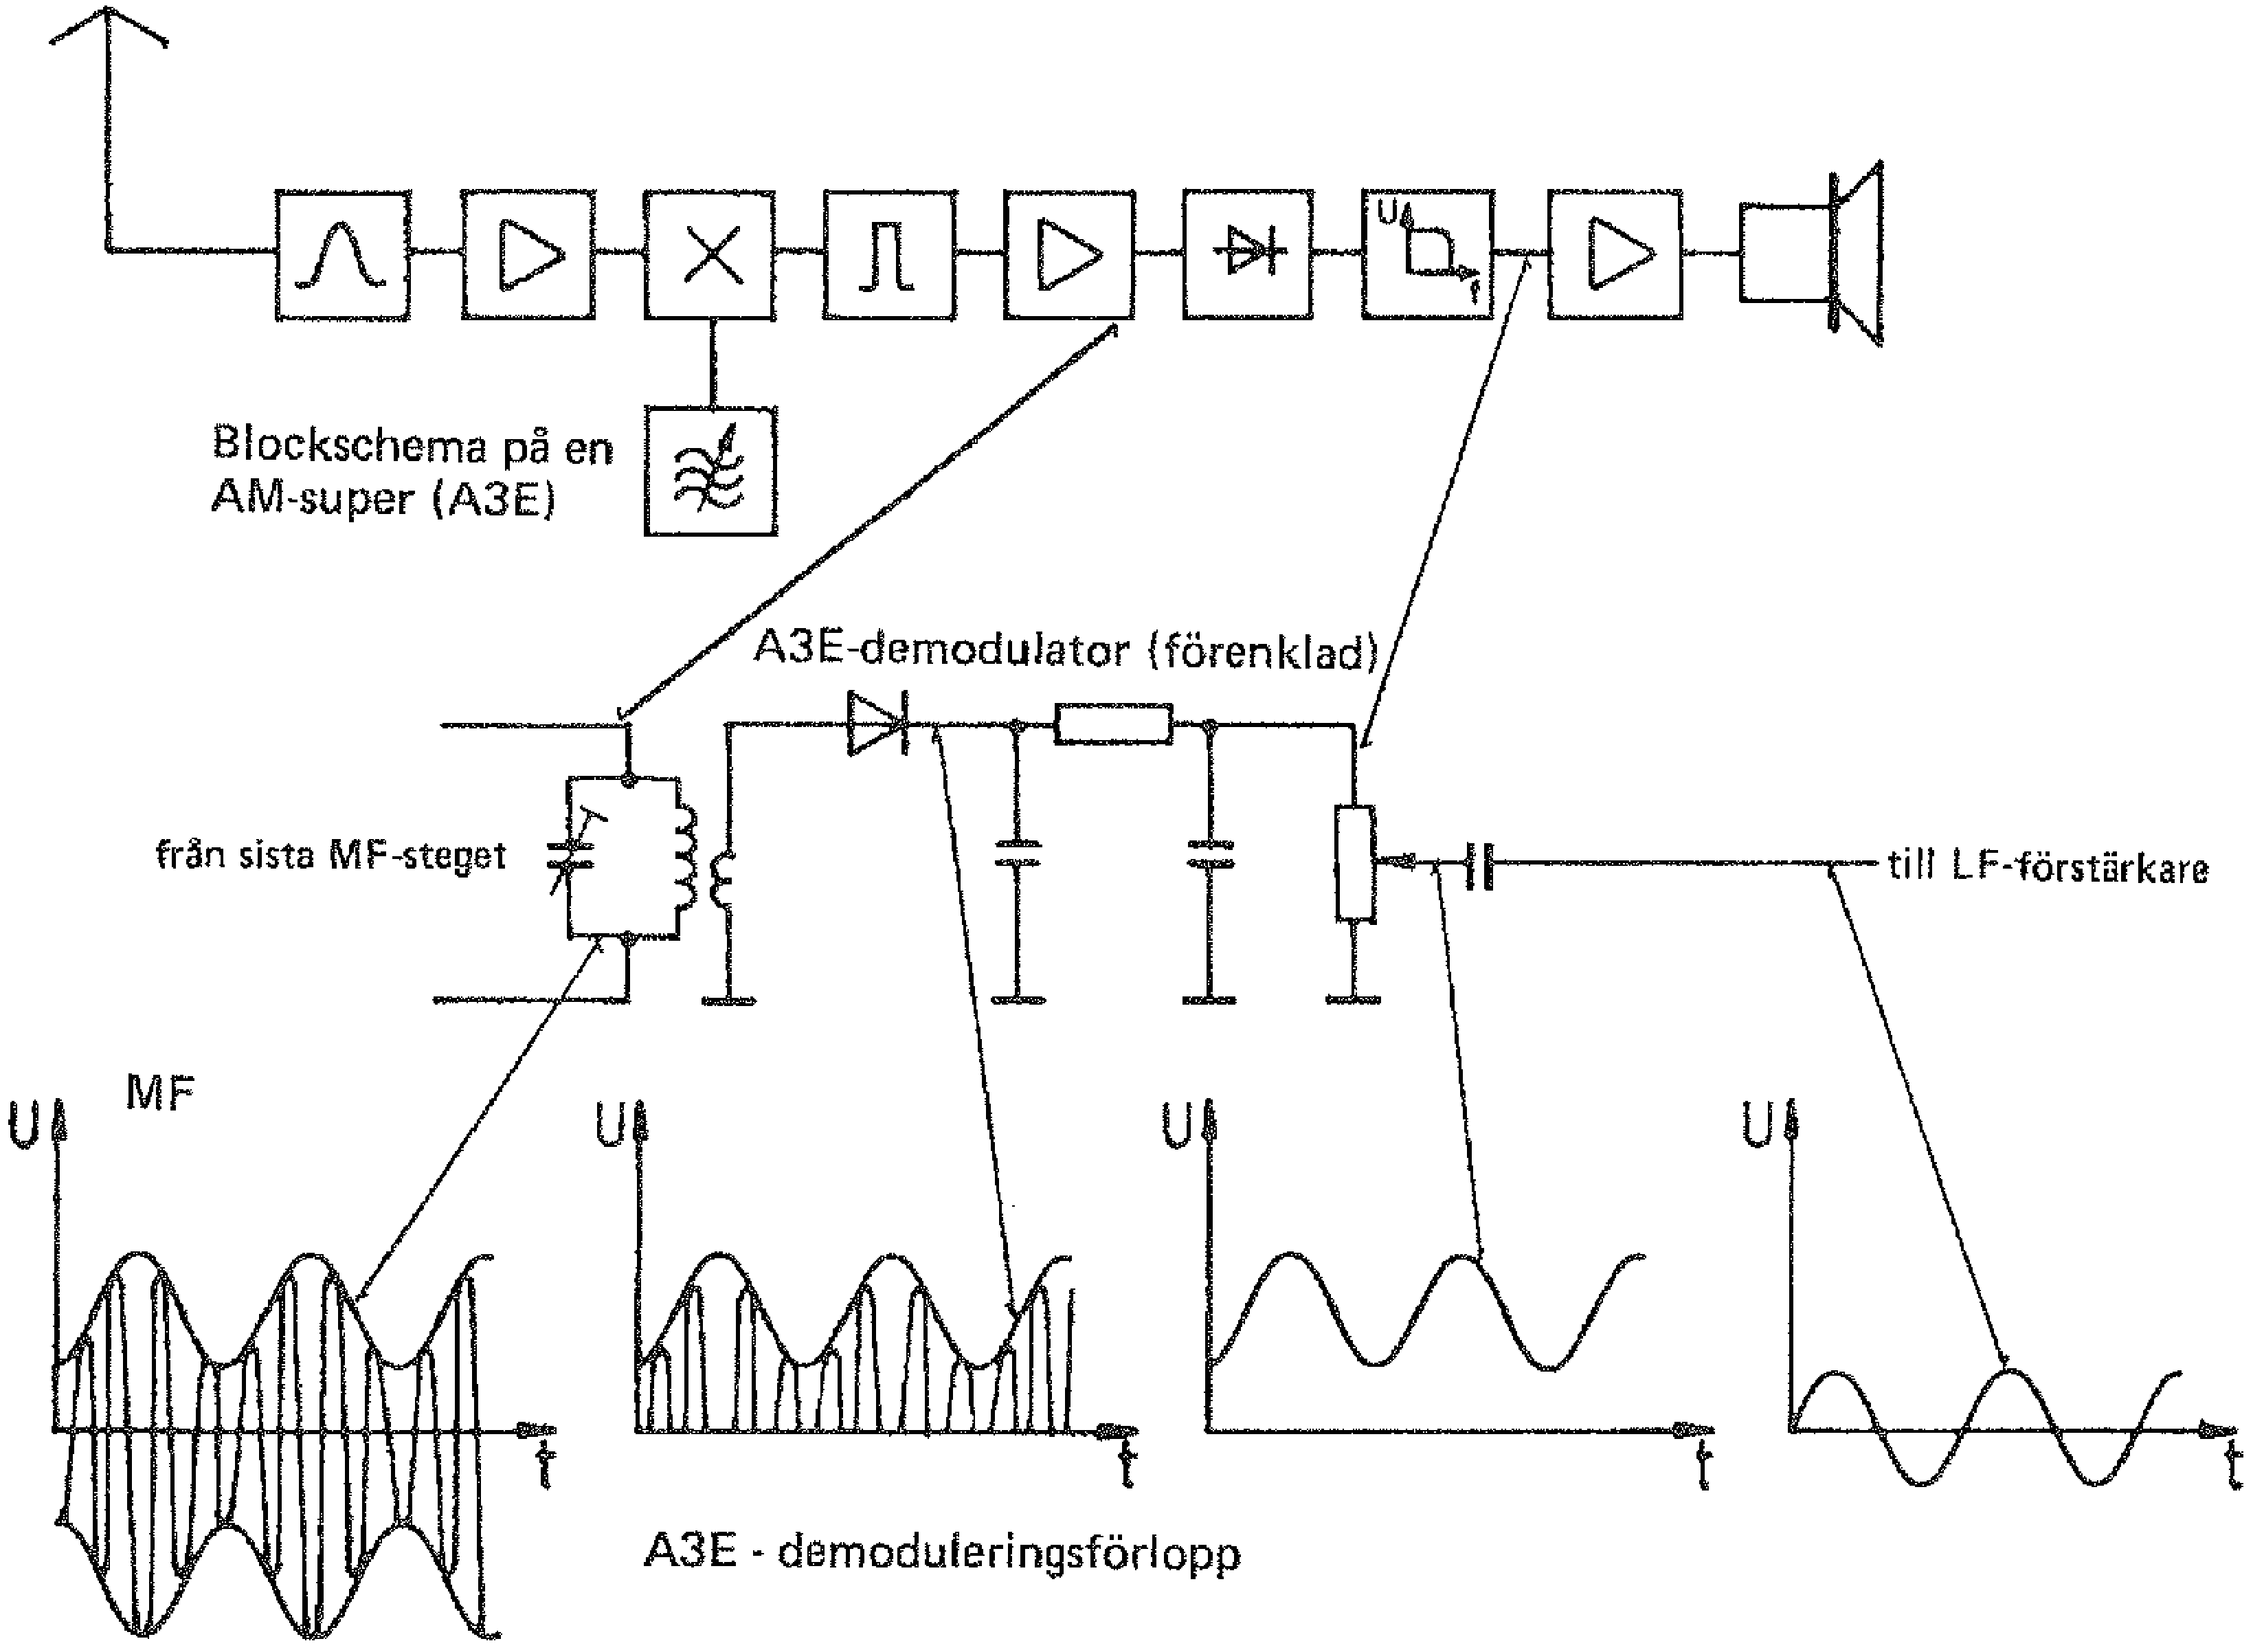
\includegraphics[width=\textwidth]{images/cropped_pdfs/bild_2_3-55.pdf}
\caption{Dioddetektorn}
\label{fig:BildII3-55}
\end{figure}

Bild \ref{fig:BildII3-55}

Bilden visar en superheterodynmottagare där den sista MF-kretsen är
induktivt kopplad till demoduleringsdioden. Den amplitudmodulerade
MF-signalen visas som ett amplitud/tid-diagram.

Dioden klipper antingen de negativa eller positiva halvvågorna,
beroende på hur den är vänd -- polariserad.

LF-signalen filtreras ut ur de högfrekventa pulserna med ett
LF-lågpassfilter.

LF-signalen är nu överlagrad på en likspänning. I talpauserna sänds
bara bärvågen och då lämnar AM-demodulatorn bara likspänning, som
skiljs från LF-förstärkaren med en kondensator. Kondensatorn släpper
bara igenom LF-signalen, som förstärks.

Dioddetektorn följer amplituden och är ett exempel på en
amplitudformsdetektor.

\subsubsection{Produktdetektorn SSB (J3E)}
\textbf{HAREC a.\ref{HAREC.a.3.5.3}\label{myHAREC.a.3.5.3}}
\index{SSB!produktdetektor}
\index{J3E!produktdetektor}
\index{produktdetektor}

\begin{figure}
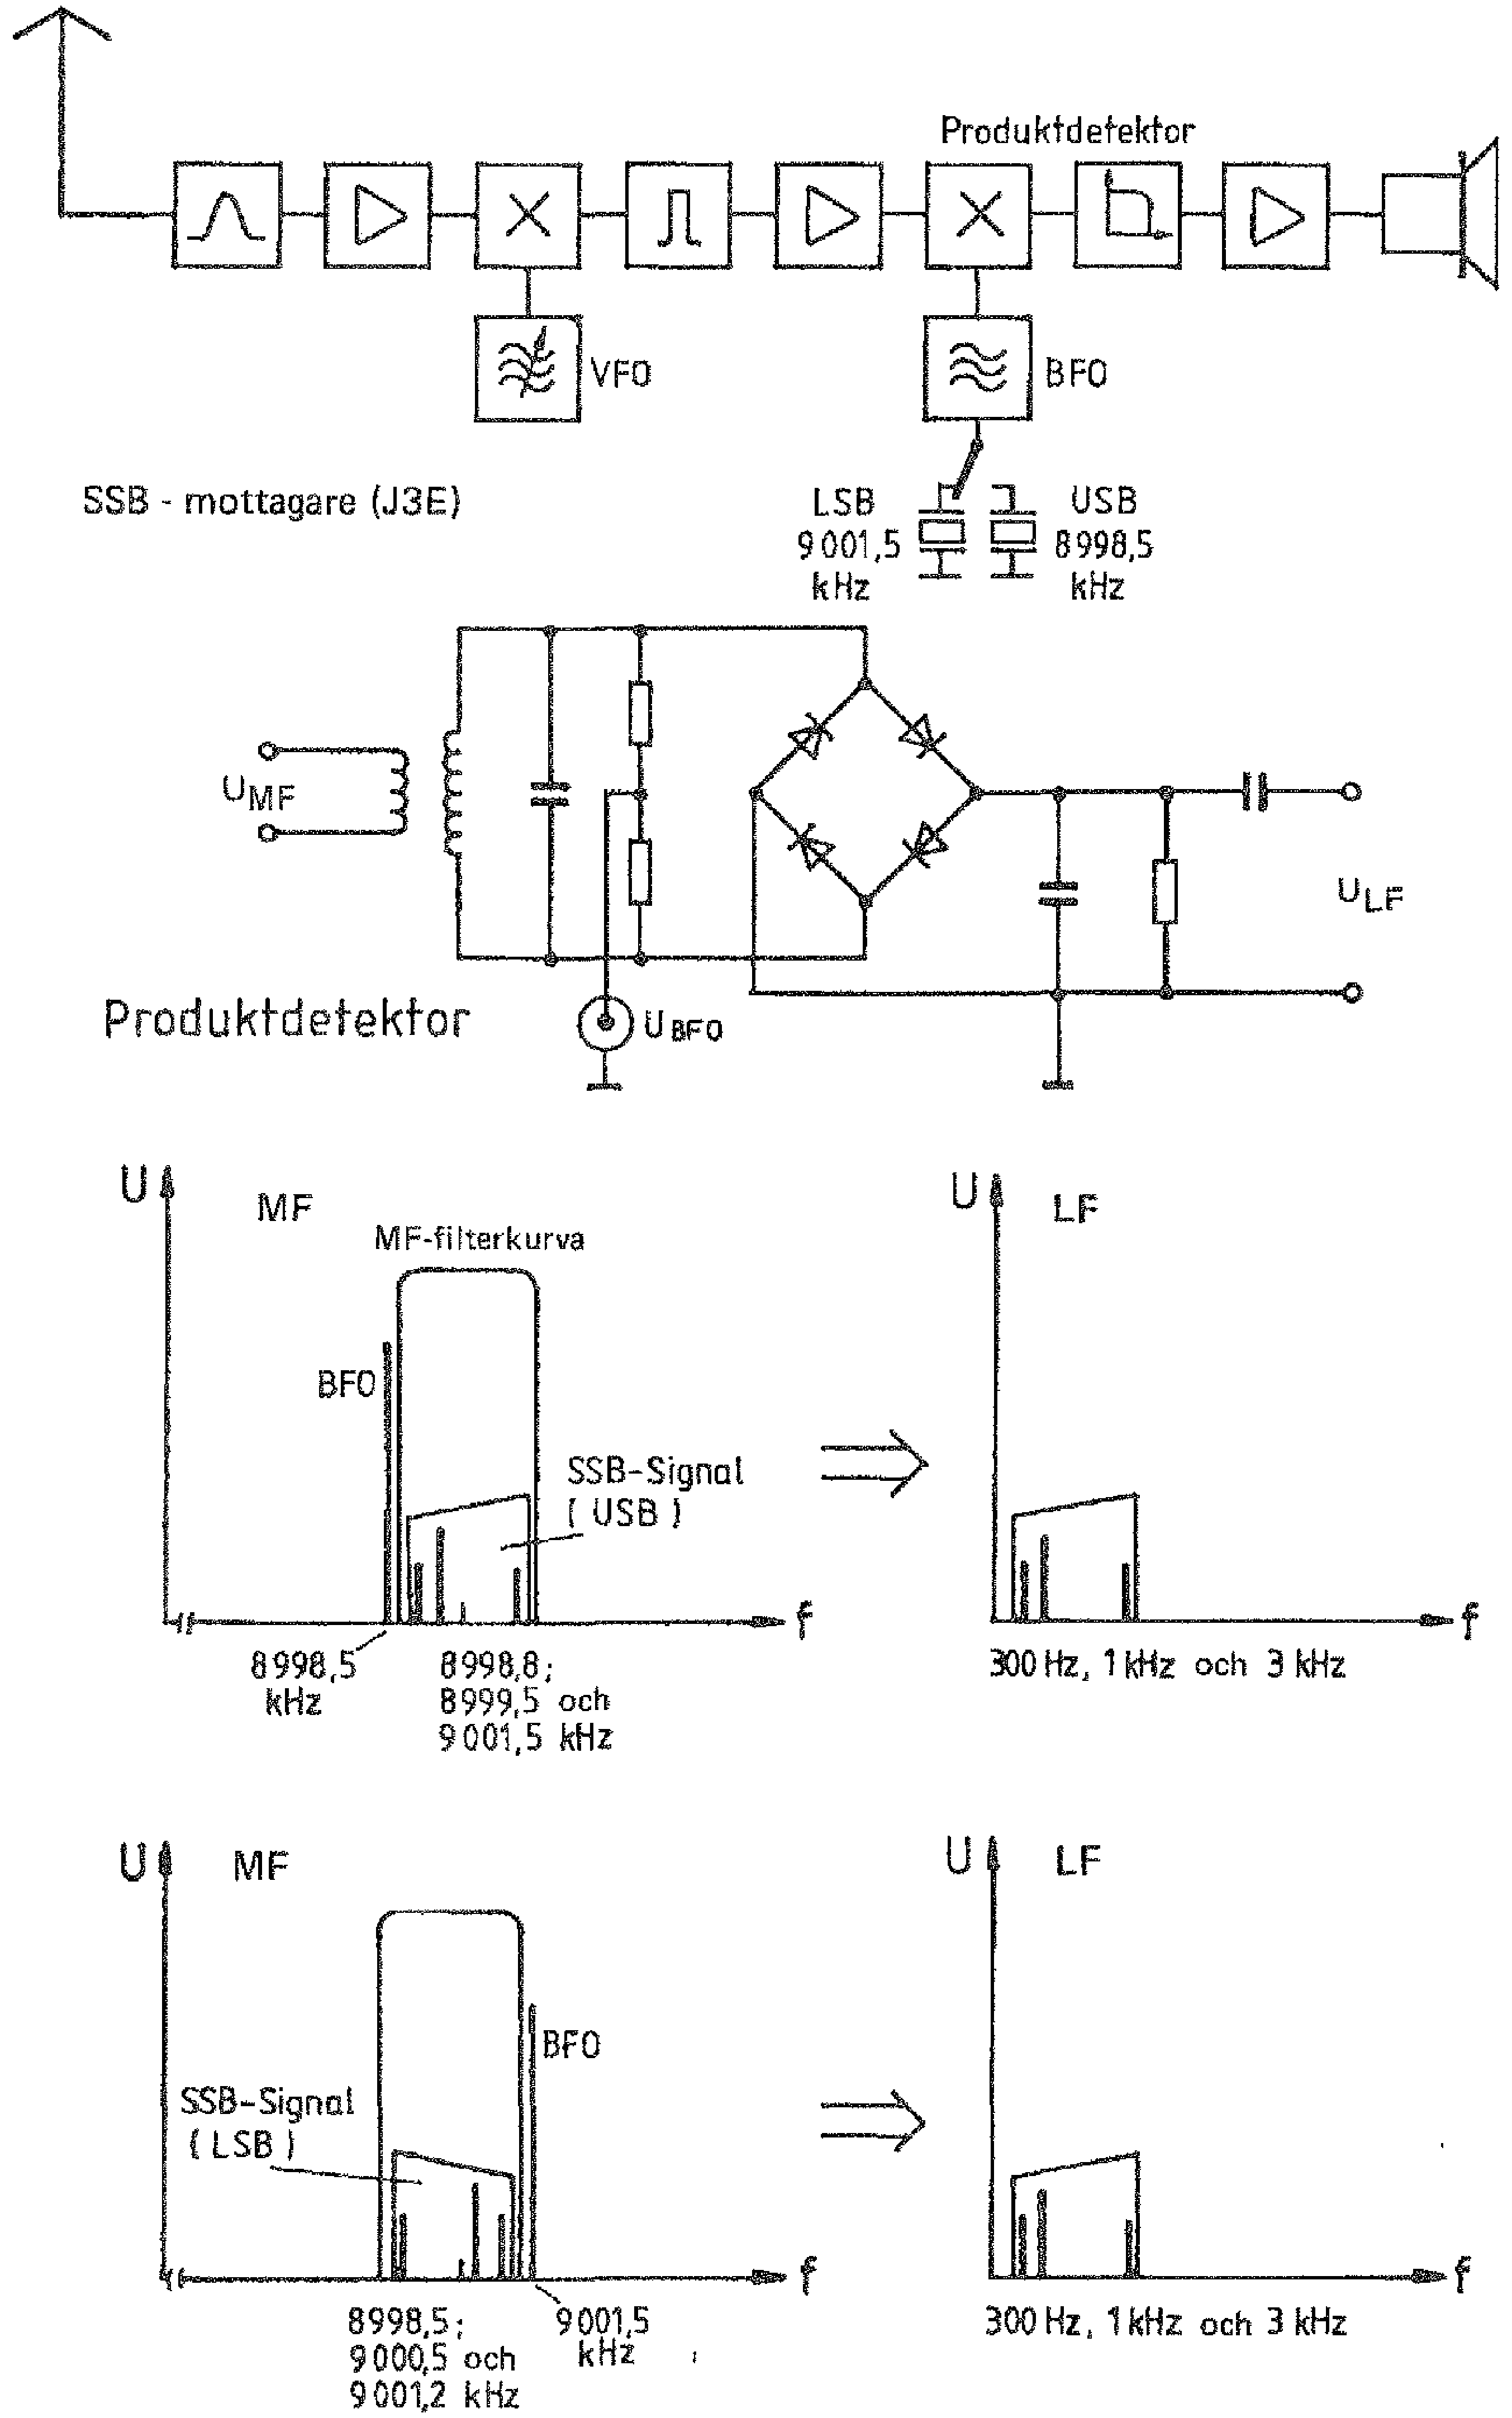
\includegraphics[width=\textwidth]{images/cropped_pdfs/bild_2_3-56.pdf}
\caption{Produktdetektor för AM (A3E) och CW (A1A)}
\label{fig:BildII3-56}
\end{figure}

Bild \ref{fig:BildII3-56}

Det finns flera metoder att demodulera en SSB-signal, såsom
fasningsmetoden, filtermetoden och den s.k. tredje
metoden. Filtermetoden är numera är den allra vanligaste och beskrivs
här.

En SSB-signal med undertryckt bärvåg består av endast ett sidband. Det
andra sidbandet och bärvågen undertrycks i sändaren.

Vid demoduleringen av SSB-signalen alstras i mottagaren en signal som
ersättning för den bärvåg som undertrycktes i sändaren. Det
undertryckta andra sidbandet ersätts inte.

I en mottagare med direktblandning blandas SSB-signalen med
VFO-signalen, varvid en del av blandningsprodukterna faller ut på
LF-nivå.

I en superheterodynmottagare däremot, blir SSB-signalen först blandad
med en VFO-signal och som resultat erhålls en mellanfrekvens MF. Den
till MF omvandlade signalen förstärks, filtreras och blandas med en
lokal BFO-signal i ytterligare en blandare, kallad
produktdetektor.
Några blandningsprodukterna faller ut på LF-nivå.
Ett lågpassfilter följer därför efter detektorn för att filtrera ut
LF-signalerna.

Numera består produktdetektorn vanligen av en ringblandare, som i ett omvänt
förlopp även kan användas vid DSB-modulering i en sändare.
Bilden visar demoduleringen av en SSB-signal som innehåller tre LF-toner.

\subsubsection{CW-/SSB-detektorer CW (A1A)}
\index{CW!detektor}
\index{SSB!detektor}
\index{A1A!detektor}
\index{detektor!CW}
\index{detektor!SSB}
\index{detektor!A1A}

Även telegrafi-signaler, även kallat CW, blir demodulerade när
MF-signalerna och BFO-signalen blandas i en produktdetektor.

Till skillnad från SSB är det vid CW inte nödvändigt med en given
skillnad mellan MF- och BFO-frekvenserna. Frekvensskillnaden påverkar
bara överlagringstonens frekvens, men inte läsligheten av
CW-budskapet.

Många moderna mottagare har en fast BFO-frekvens för CW, som ger en
800~Hz-ton vid rätt frekvensinställning. I stället för lågpassfiltret
för SSB, används ibland ett bandpassfilter, som bara släpper igenom
CW-signaler i frekvensområdet 800~Hz -- en idealfrekvens för god
läsbarhet av morsetecken.

\subsection{FM- och PM-detektorer}
\textbf{
HAREC a.\ref{HAREC.a.3.5.4}\label{myHAREC.a.3.5.4},
 a.\ref{HAREC.a.4.2.4}\label{myHAREC.a.4.2.4},
 a.\ref{HAREC.a.4.3.5}\label{myHAREC.a.4.3.5}
}
\index{FM-detektor}
\index{FM!detektor}
\index{detektor!FM}
\index{PM-detektor}
\index{PM!detektor}
\index{detektor!PM}

\begin{figure}
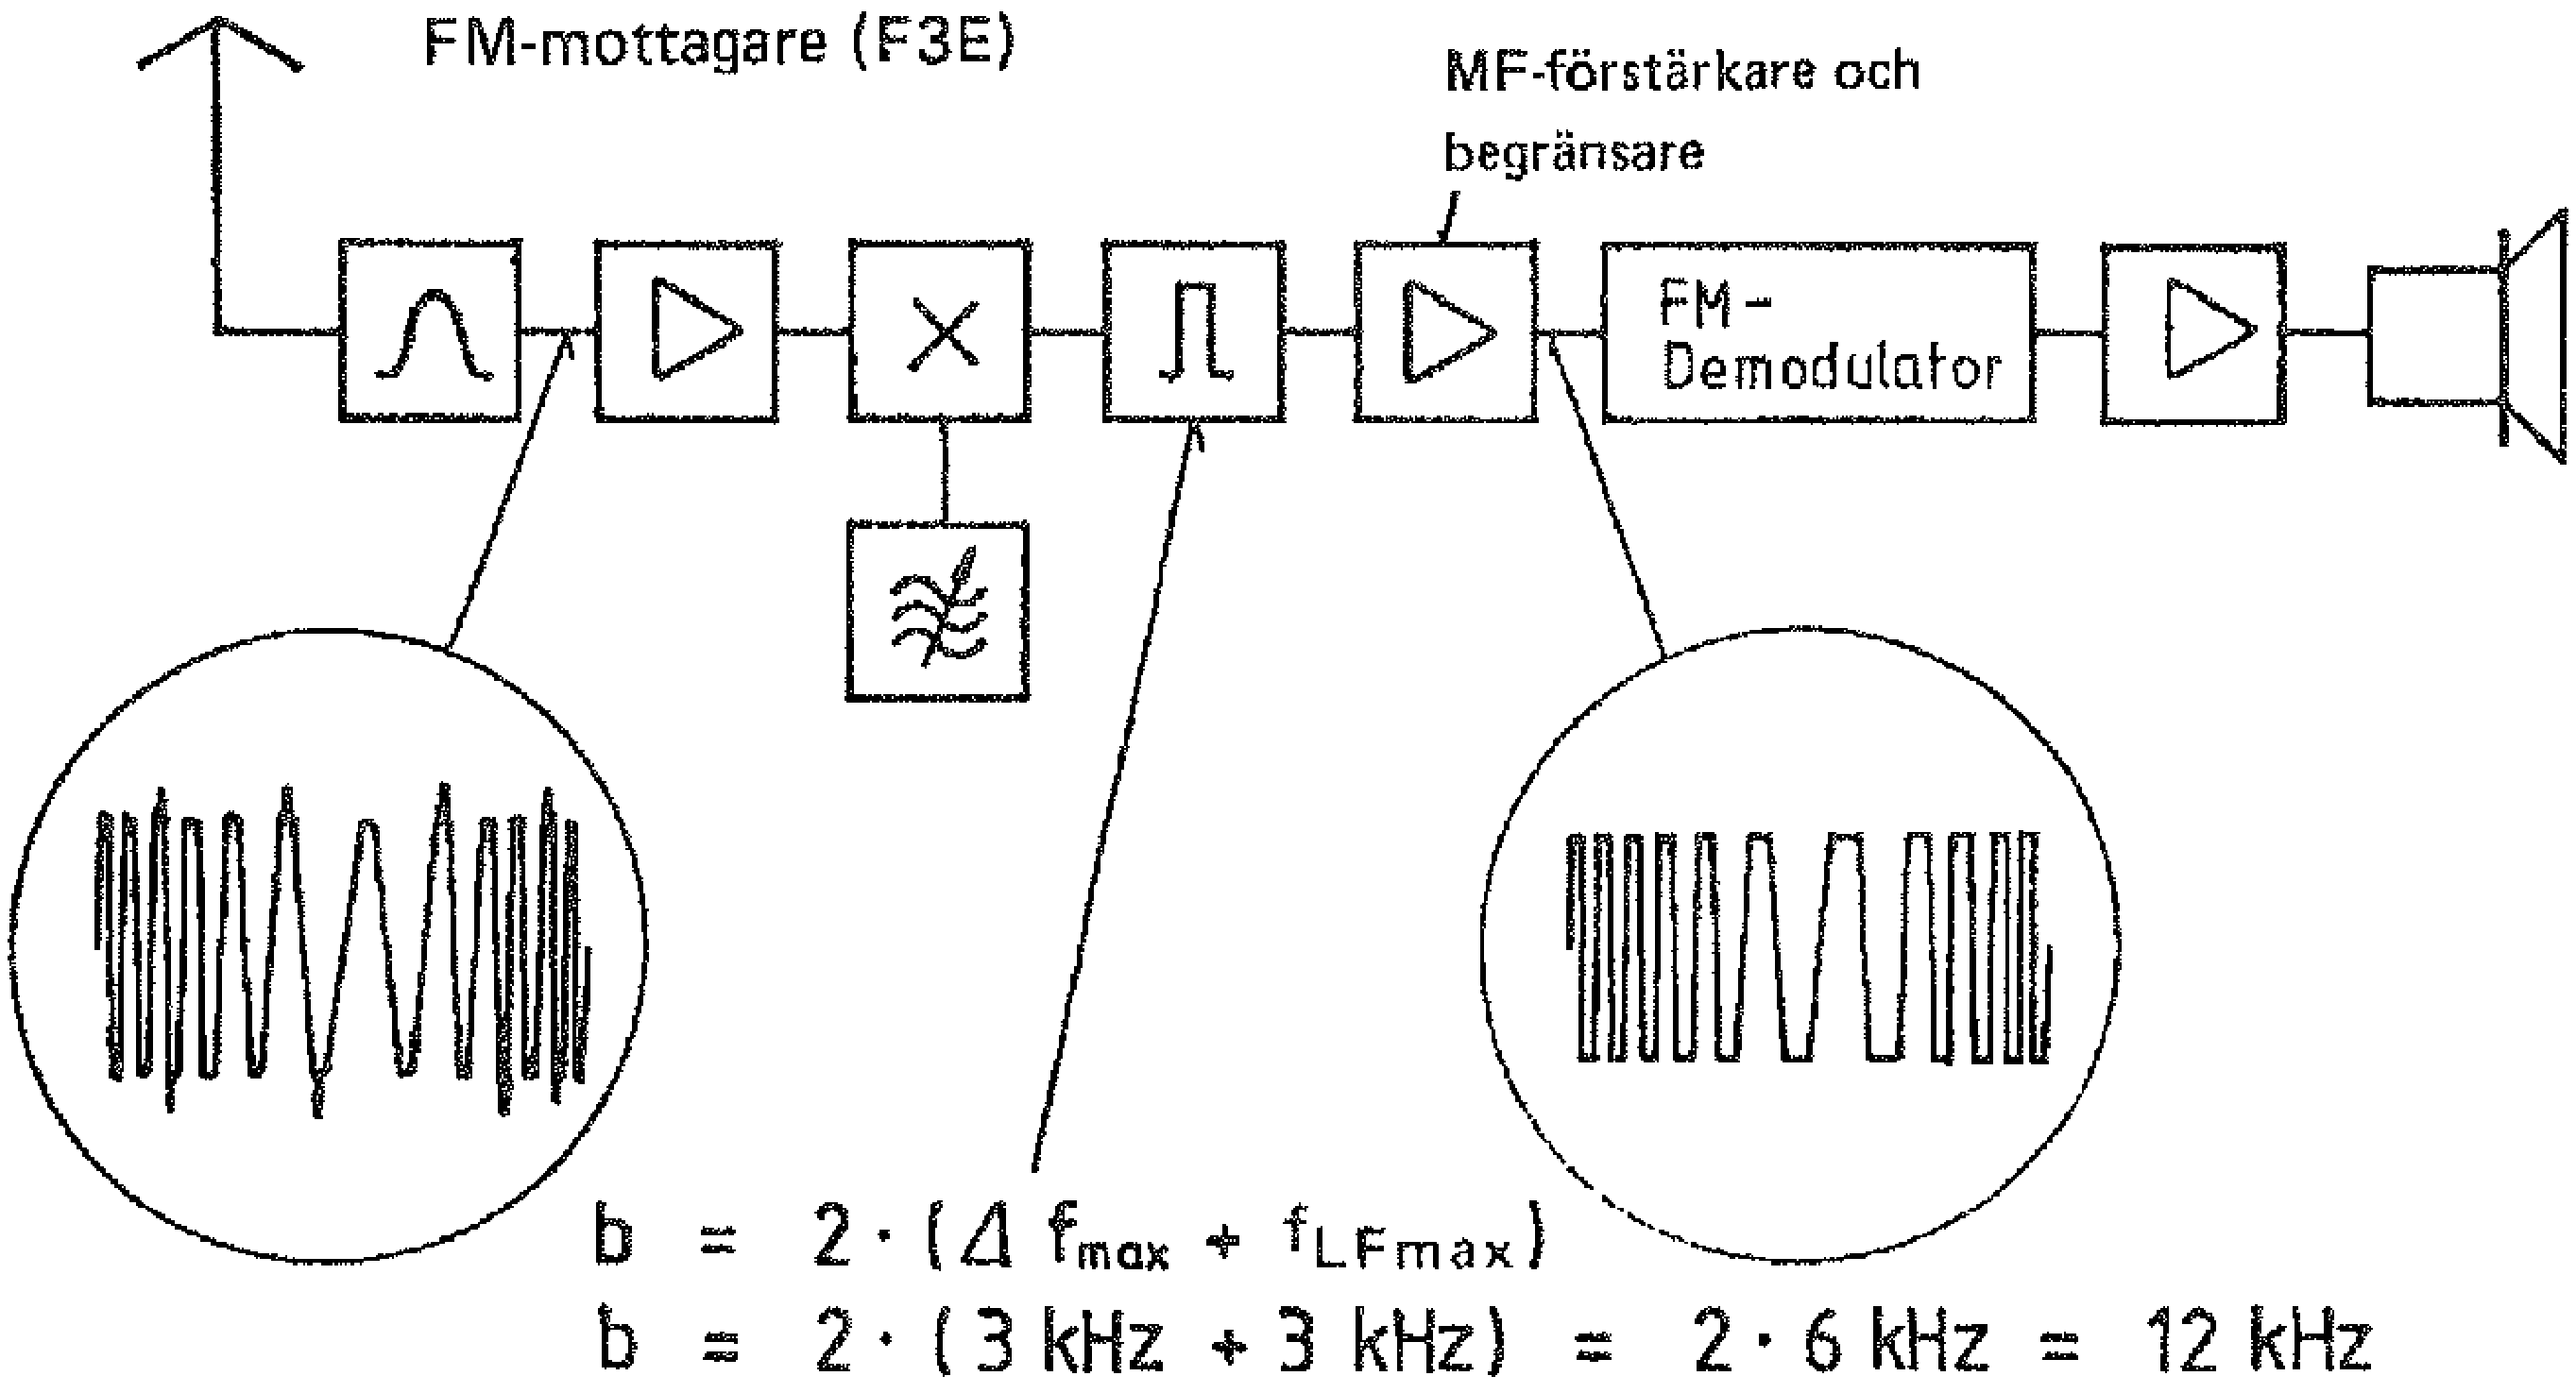
\includegraphics[width=\textwidth]{images/cropped_pdfs/bild_2_3-57.pdf}
\caption{Amplitudbegränsning vid FM-mottagning}
\label{fig:BildII3-57}
\end{figure}

Bild \ref{fig:BildII3-57}

Vid vinkelmodulering överförs informationen enbart genom frekvens-
eller fasvariationer i bärvågen. De amplitudvariationer som kan uppstå
före demoduleringen är ej önskvärda i detta sändningsslag. Av den
anledningen finns i FM-mottagare en amplitudbegränsare (limiter) före
diskriminatorn (se följande bild). Frekvensvariationerna i den
FM-modulerade signalen omvandlas därefter av detektorn till
LF-spänning som motsvarar det utsända talet.

\begin{figure}
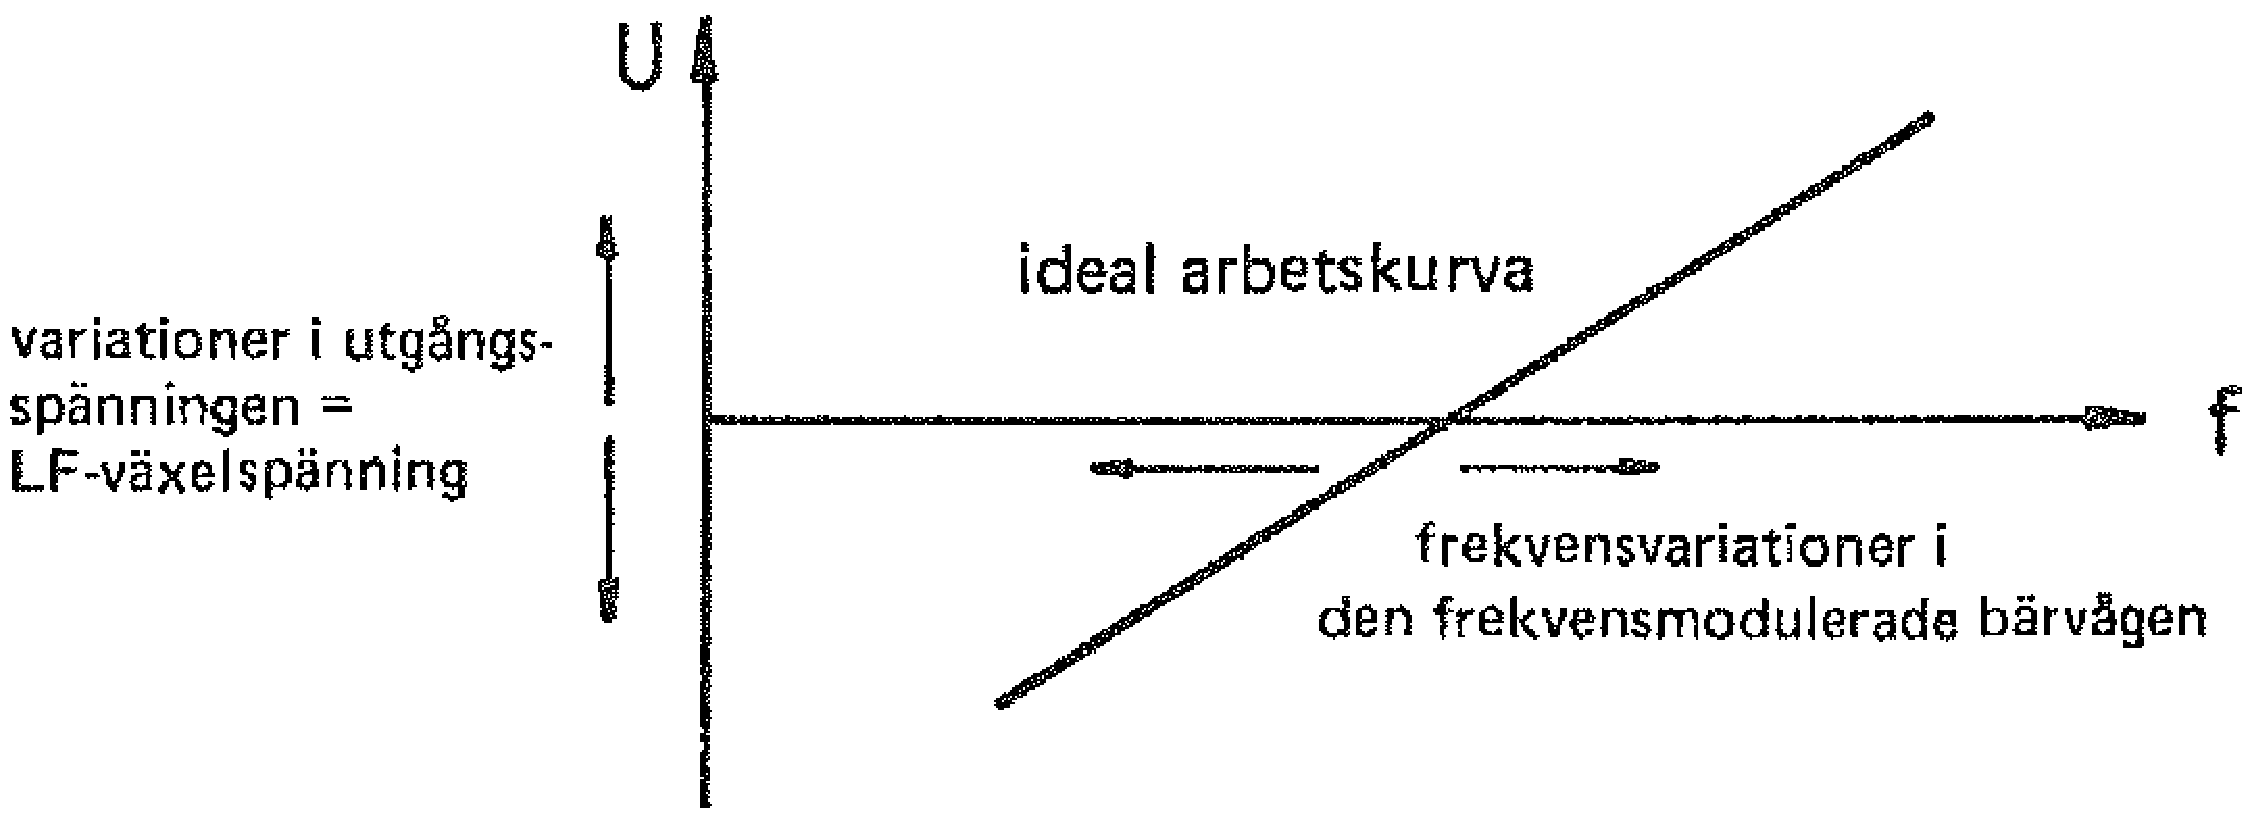
\includegraphics[width=\textwidth]{images/cropped_pdfs/bild_2_3-58.pdf}
\caption{Ideal arbetslinje för diskriminator}
\label{fig:BildII3-58}
\end{figure}

Bild \ref{fig:BildII3-58}

Demoduleringen ska ske med mottagaren inställd mitt på avsedd
sändarfrekvens. Ett hjälpmedel för det är en indikator, som vid rätt
inställning visar värdet noll. Positivt eller negativt utslag anger
att inställningen är för högt respektive för lågt i frekvens. En sådan
indikator fanns i tidiga FM-mottagare. Nu används i stället en AFC
(Automatic Frequency Control) som själv ställer in mottagaren
om sändarfrekvensen är tillräckligt nära.

\subsubsection{Slope-detektorn -- Diskriminatorn FM (F3E)}
\index{slope-detektorn}
\index{detektor!slope-detektorn}
\index{FM!slope-detektorn}
\index{FM-diskriminator}
\index{detektor!FM}
\index{detektor!F3E}
\index{FM!detektor}
\index{F3E!detektor}

\begin{figure}
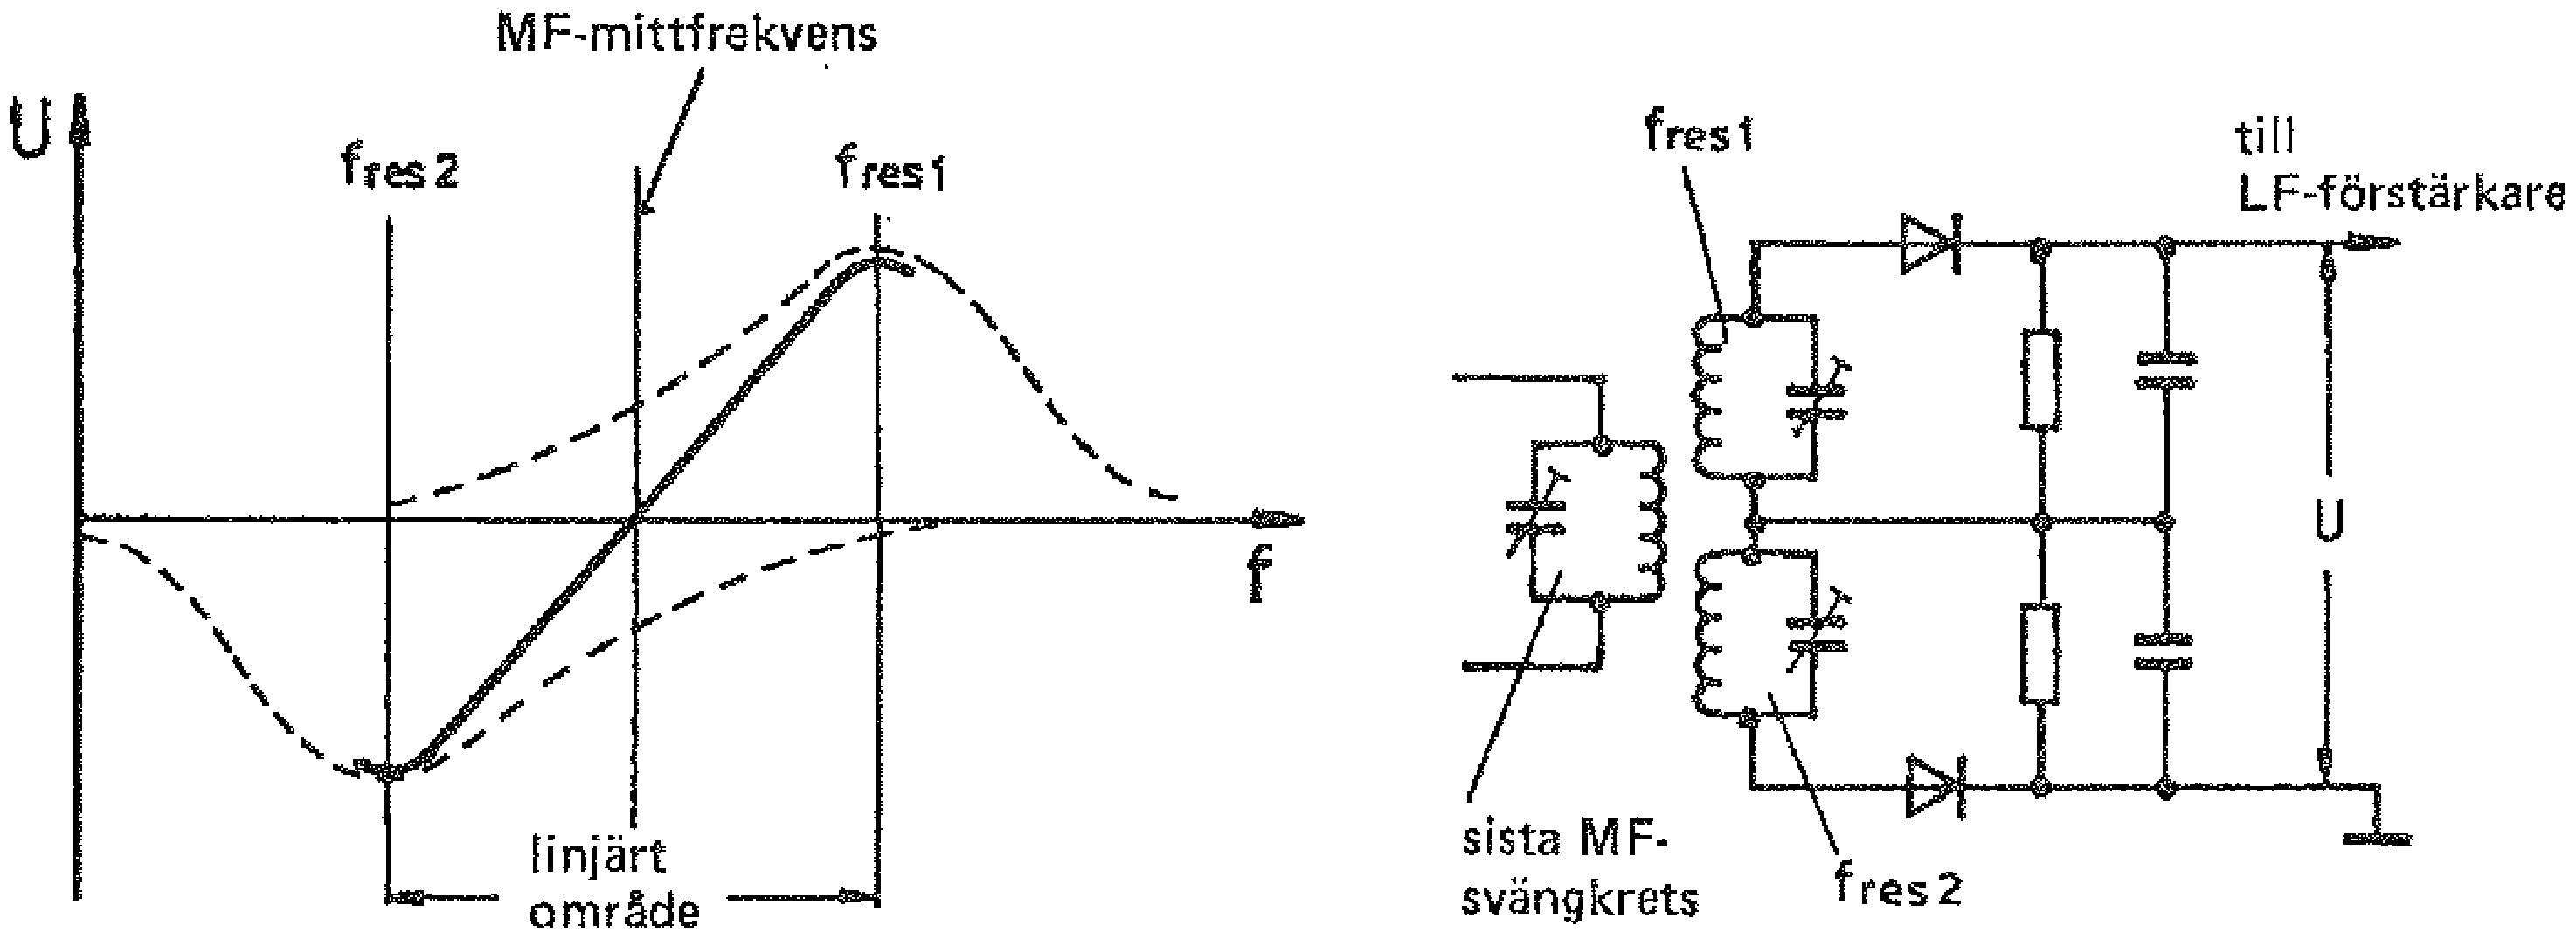
\includegraphics[width=\textwidth]{images/cropped_pdfs/bild_2_3-59.pdf}
\caption{Slope-detektorn}
\label{fig:BildII3-59}
\end{figure}

Bild \ref{fig:BildII3-59}

Två svängningskretsar är kopplade induktivt till den sista
MF-kretsen. Resonansfrekvensen för dessa båda kretsar är något högre
respektive något lägre än mellanfrekvensen. De signalspänningar som
uppträder över svängningskretsarna likriktas och seriekopplas med
varandra med motsatt polaritet.

När de båda svängningskretsarna matas med samma frekvens, kommer
likspänningarna att ta ut varandra. När frekvensen avviker uppåt i
frekvens, kommer kretsen med den högre resonansfrekvensen i kraftigare
svängning än den andra kretsen och avger högre likriktad spänning. När
frekvensen avviker nedåt i frekvens, skiftar de båda kretsarna roller,
och den resulterande likriktade spänningen skiftar till motsatt
polaritet.

Vid växelvisa frekvensändringar i MF, över och under vilofrekvensen,
blir resultatet en växelspänning ut från likriktarnas utgångsfilter,
som är LF-signalen.

\subsubsection{Foster-Seeley diskriminatorn}
\index{Foster-Seely diskriminator}
\index{detektor:Foster-Seely diskriminator}
\index{FM:Foster-Seely diskriminator}

\begin{wrapfigure}[12]{5}{0.5\textwidth}
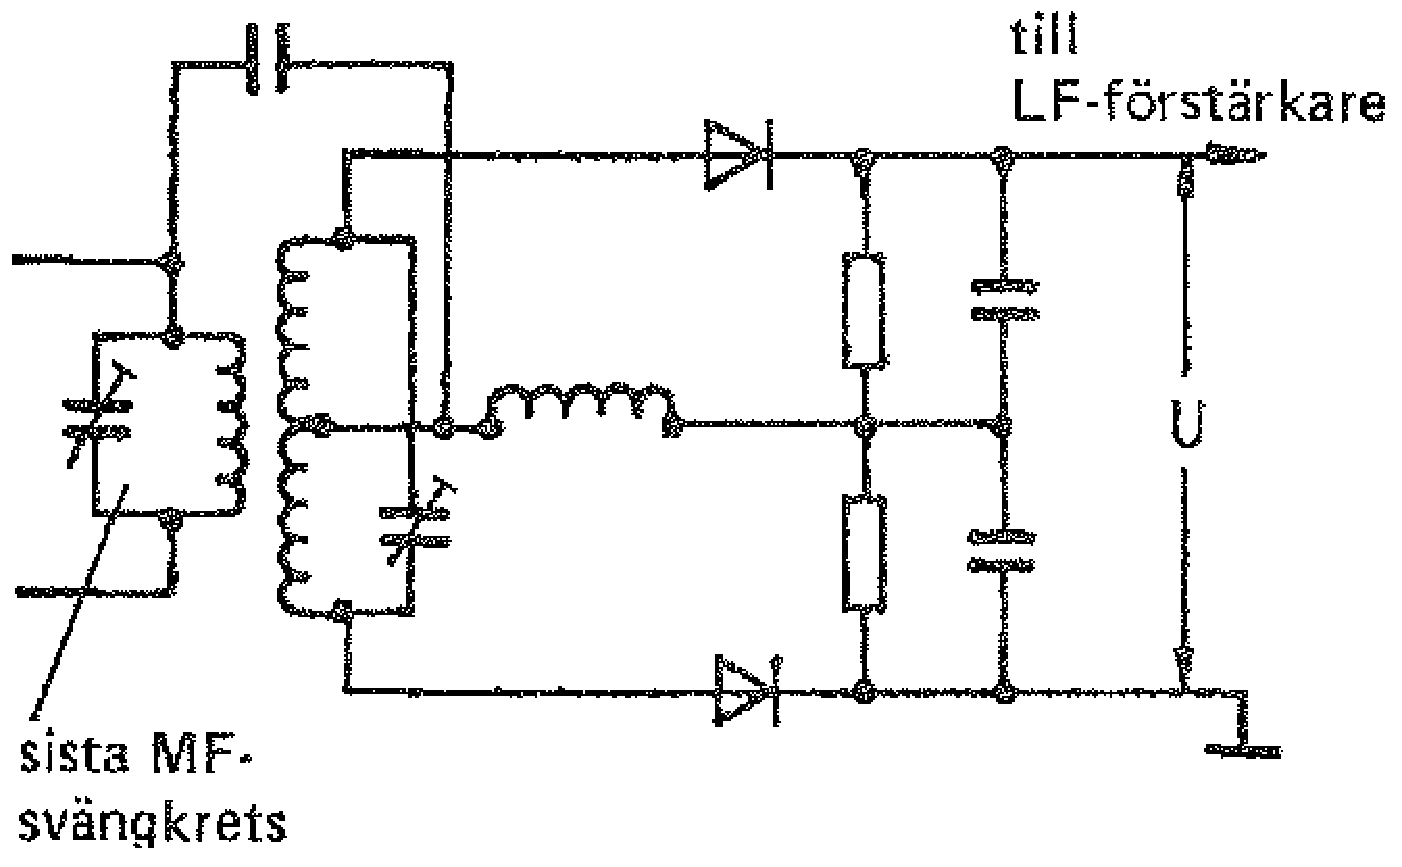
\includegraphics[width=0.5\textwidth]{images/cropped_pdfs/bild_2_3-60.pdf}
\caption{Foster-Seeley detektorn}
\label{fig:BildII3-60}
\end{wrapfigure}

Bild \ref{fig:BildII3-60}

Denna tidiga demodulator har god linjäritet, om den föregås av en god
amplitudbegränsare, men har tämligen dålig känslighet.

Sista MF-förstärkarsteget avslutas med en transformator vars båda
lindningar ingår i svängningskretsar avstämda till MF. MF-signalen
överförs från primär- till sekundärsidan dels med induktion och dels
med en kondensator till mitten av sekundärlindningen. Signalen delas på
så sätt i två grenar med en fasförskjutning av +90\degree resp. -90\degree.
Signalerna i grenarna likriktas varför sig och sammanlagras i ett
RC-nät.

Om MF-signalen inte devierar så är LF-spänningen i grenarna lika, men
eftersom grenspänningarna har motsatt polaritet så tar de ut varandra
och LF-signalen blir noll.  När MF-frekvensen devierar av modulering,
så ökar signalamplituden i den ena grenen och minskar i den
andra. LF-signalens amplitud blir då proportionell med
frekvensdeviationen.

\subsubsection{Räknardiskriminatorn}
\index{räknardiskriminator}
\index{FM!räknardiskriminator}
\index{detektor!räknardiskriminator}

\begin{figure}
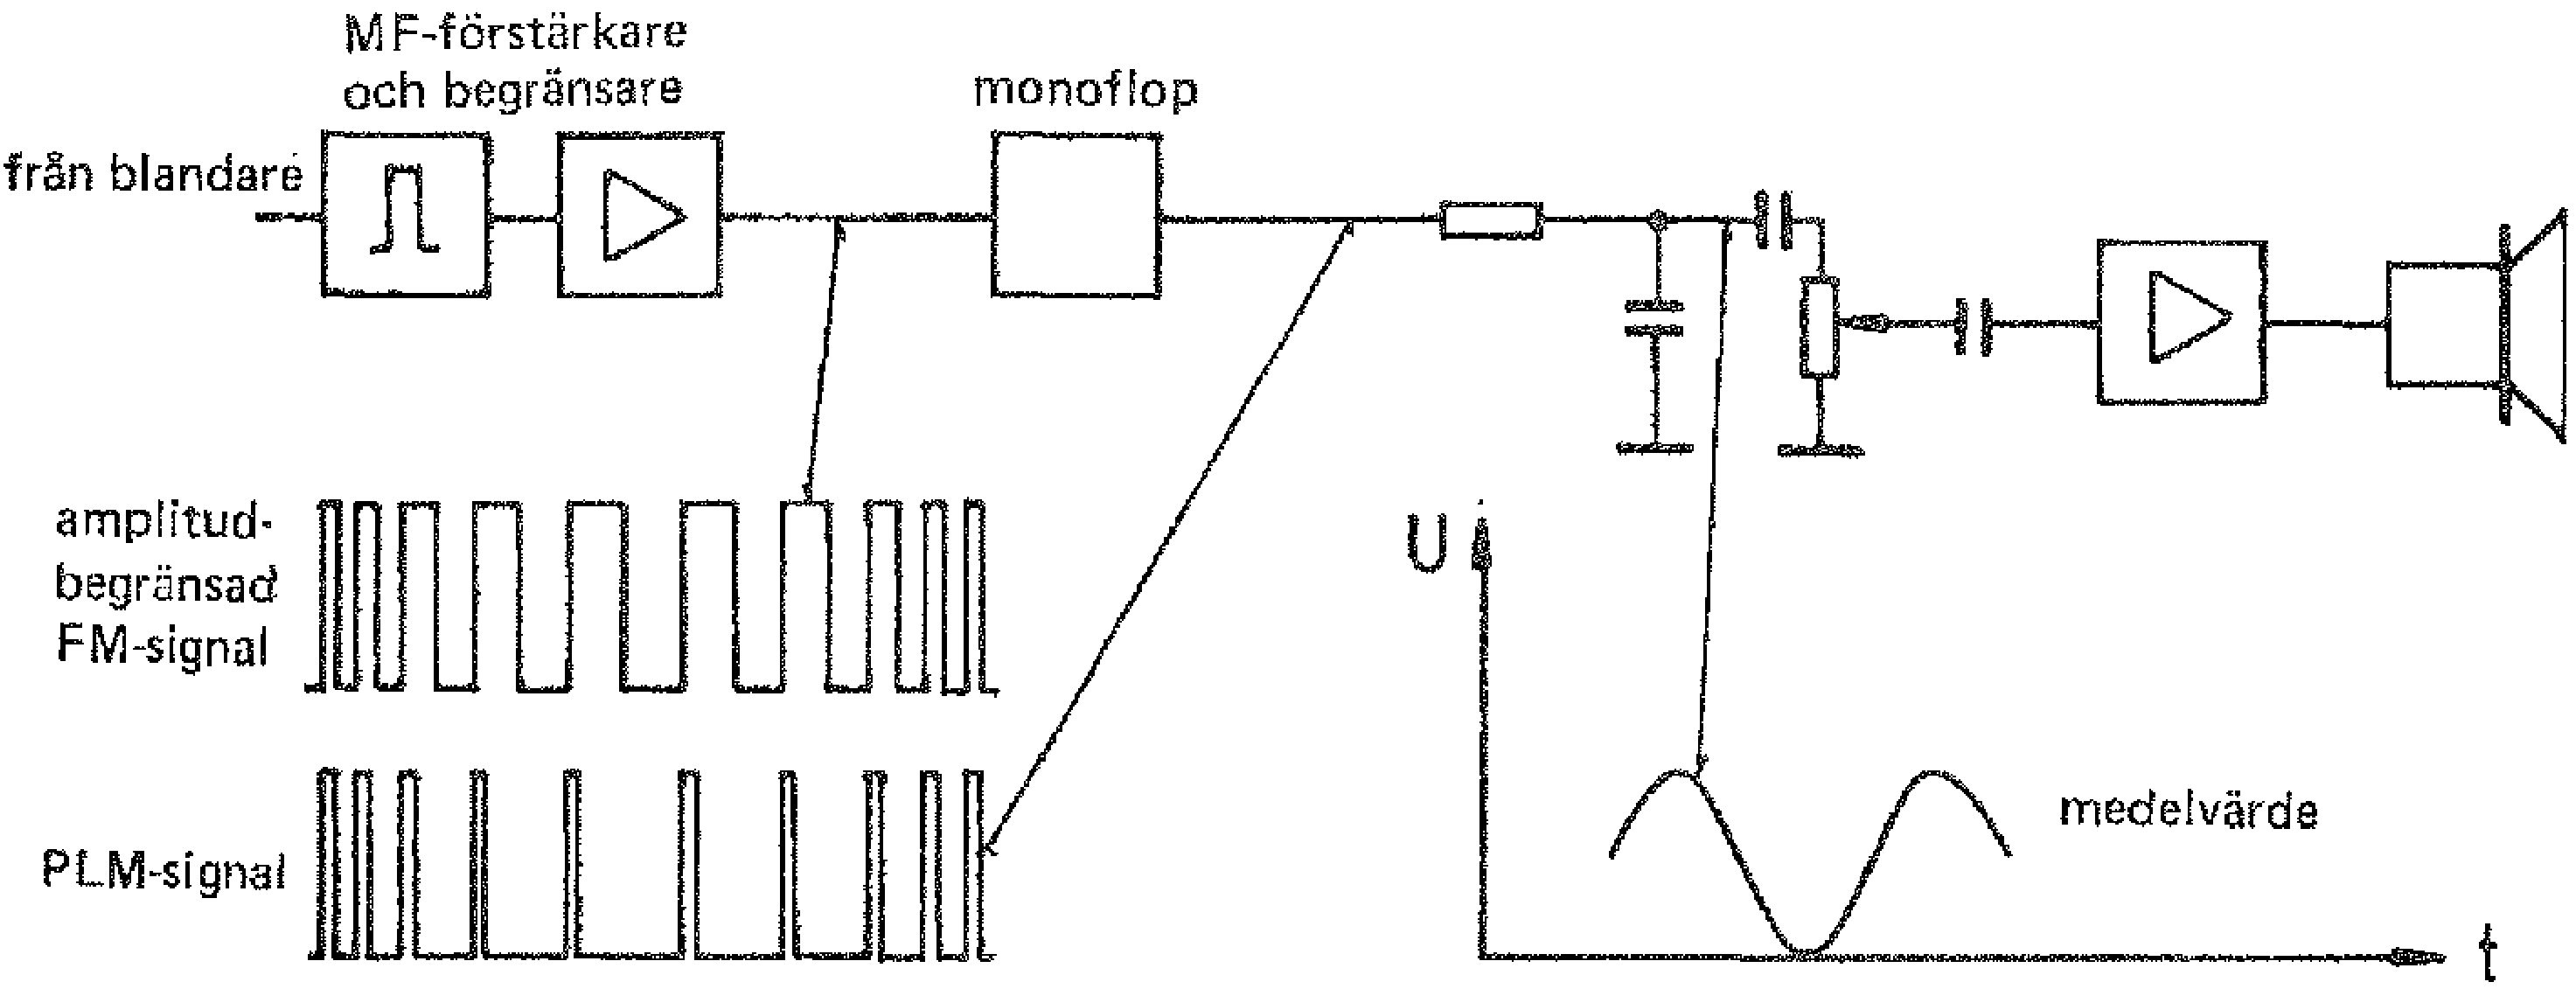
\includegraphics[width=\textwidth]{images/cropped_pdfs/bild_2_3-61.pdf}
\caption{Räknardiskriminatorn}
\label{fig:BildII3-61}
\end{figure}

Bild \ref{fig:BildII3-61}

En mono-floppvippa påverkas att slå över av fyrkantspulserna från de
amplitudbegränsade FM-signalerna.

En sådan vippa är en digitalkoppling som, när den matas med en
godtyckligt lång spänningspuls, ändå kommer att leverera en
spänningspuls med konstant längd. För varje positiv halvvåg levererar
mono-floppvippan en impuls av konstant längd. Tidsavståndet mellan
pulserna kommer att vara proportionella till FM-signalens
frekvens. Vid varierande frekvens kommer impulserna med varierande
tidsavstånd. Ett lågpassfilter filtrerar ut lågfrekvensen ur signalen
och en pulserande likspänning kvarstår. Med denna likspänning laddas
kondensatorn upp till ett medelvärde. Vid en högre frekvens av lika
långa pulser blir medelvärdet högre än vid en lägre pulsfrekvens.

Svängningarna på likspänningen är LF-signalen, överlagrad på en
likspänning. Utan en mono-flopp med lika långa pulser hade medelvärdet
varit konstant. Man kan säga att FM-signalen blivit omvandlad till en
PLM-signal (pulslängdmodulerad signal).

\subsubsection{PLL-demodulatorn}
\index{PLL-demodulator}
\index{PLL!demodulator}
\index{FM!PLL-demodulator}
\index{detektor!PLL-demodulator}

\begin{figure}
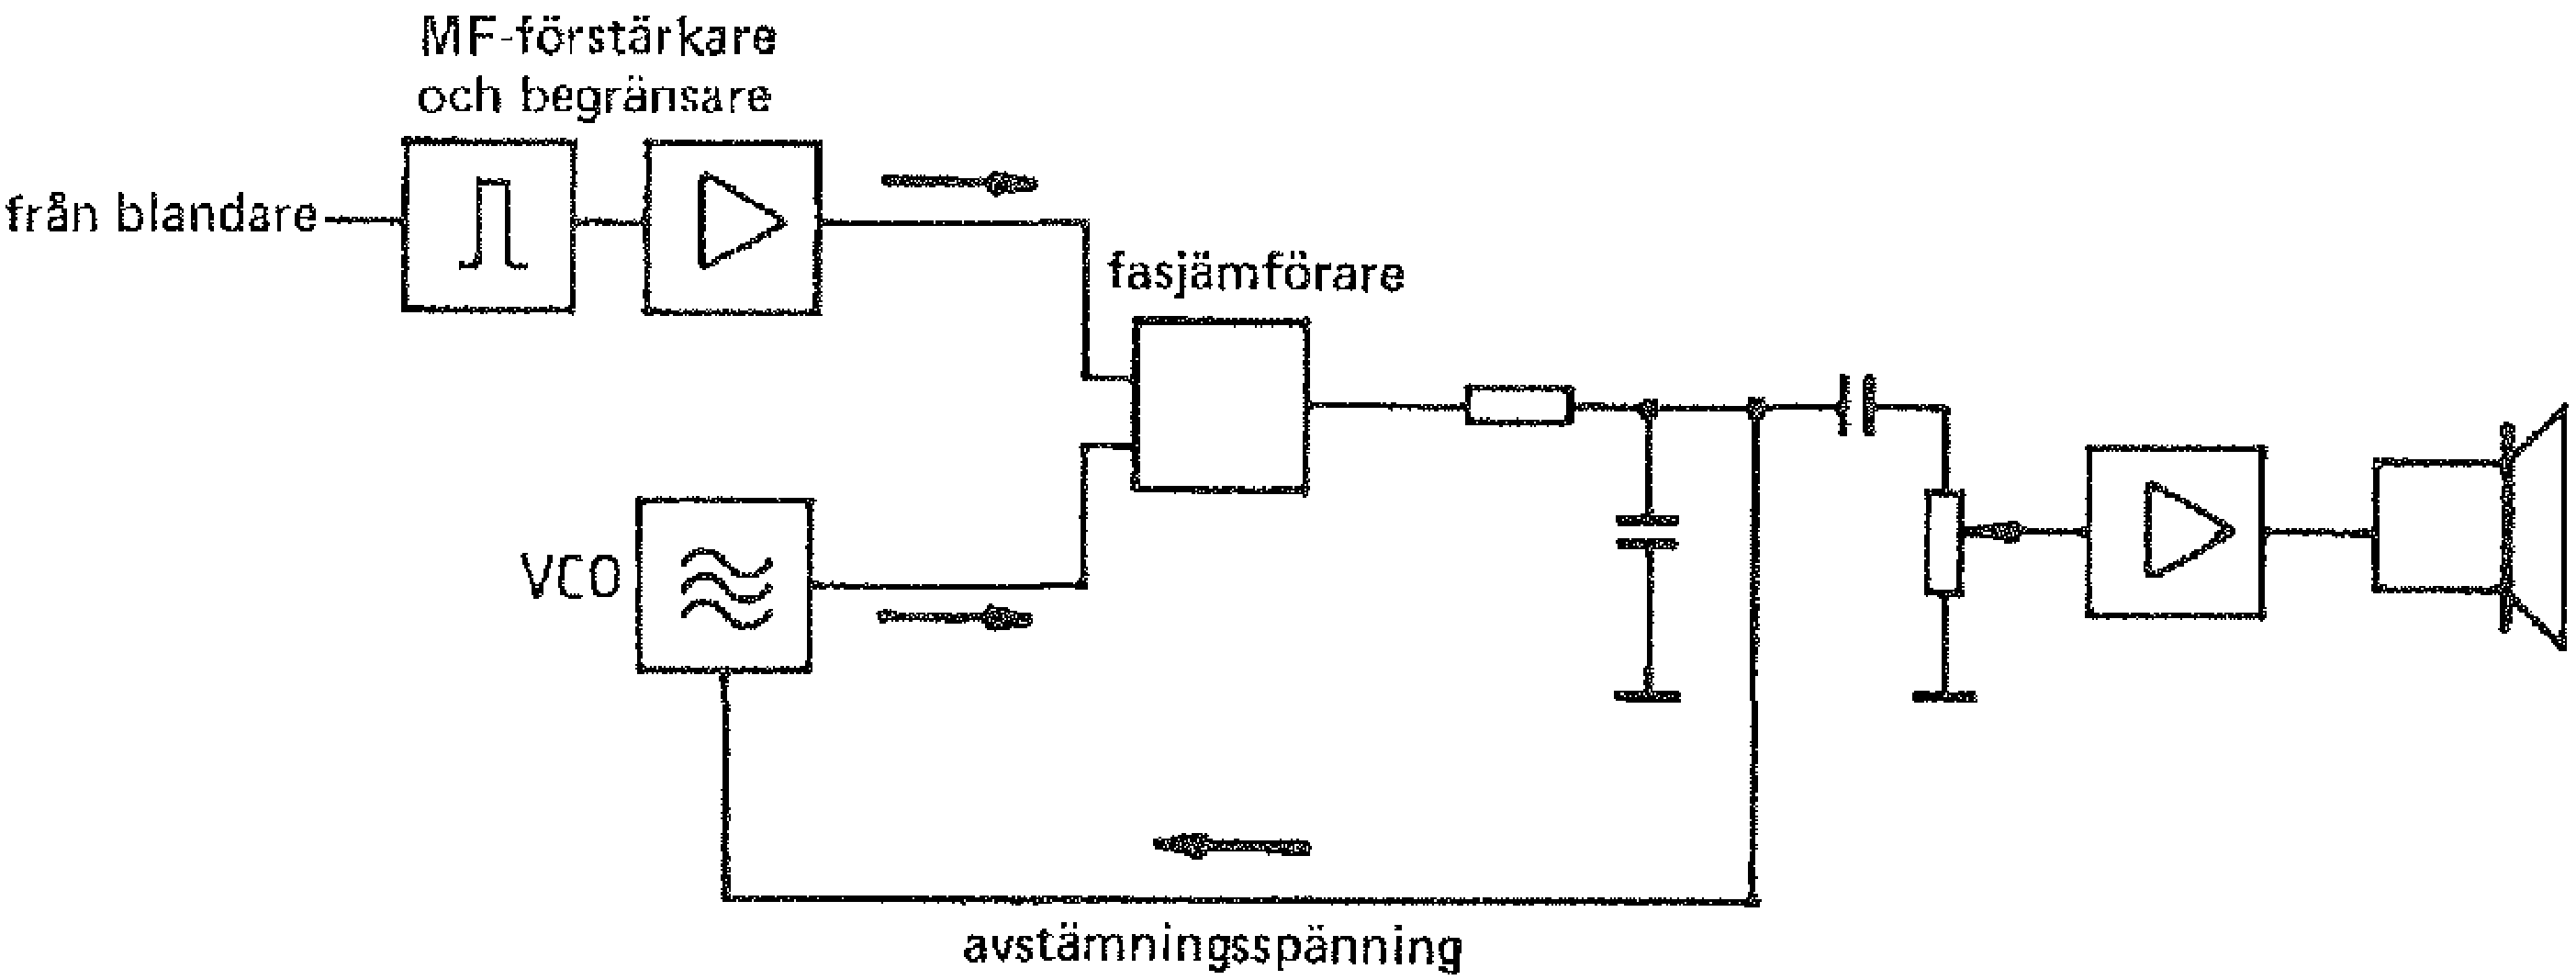
\includegraphics[width=\textwidth]{images/cropped_pdfs/bild_2_3-62.pdf}
\caption{PLL-demodulatorn}
\label{fig:BildII3-62}
\end{figure}

Bild \ref{fig:BildII3-62}

Den frekvensmodulerade MF-signalen och en VCO-signal matas in i en
fasjämförare. VCO-frekvensen följer frekvensändringarna FM-signalen
Avstämningsspänningen för VCO är en likspänning. Den modulerande
LF-spänningen är överlagrad på denna likspänning.

LF-frekvenserna är för låga för att kunna reglera VCO-frekvensen, men
via en kondensator kan de styra LF-förstärkaren.

De båda sista metoderna lämpar sig speciellt för demodulering av
F1-signaler. F1-signaler kan ''demoduleras'' i en SSB-mottagare eftersom
det uppstår en rytmisk svängning i tonhöjden. Denna frekvensmodulerade
ton kan sedan demoduleras på sätt som beskrivits.

Det finns ytterligare sätt att demodulera FM-signaler. Gemensamt för
alla är, att de fungerar bättre ju lägre mellanfrekvensen är.  Därför
utförs de flesta FM-mottagare som dubbel- eller trippelsuprar, med låg
MF.
